\chapter{A/D and D/A Converters}
\section{Introduction}

A \emph{converter} is an electronic device that transforms a signal:
\begin{itemize}
	\item From an analog to a digital signal (ADC)
	\item From a digital to an analog signal (DAC)
\end{itemize}
An \emph{analog} signal is continuous over time, i.e. it has a value for every time $t$, and can take any value (typically between a minimum and maximum value).\\
A \emph{digital} signal can only be equal to a certain number $S_i$, with usually $0 \le S_i \le 2^n - 1$. $S_i$ can thus be stored as a binary number of $n$ bits. The number $S_i$ is related to the value $V_i$ of the sample: $V_i = (V_{max} - V_{min}) \frac{S_i}{2^n}$. The distance between two successive levels is one LSB or least significant bit.\\
Furthermore, a digital signal is not continuous over time: it represents a signal at specific moments in time. The period between these time instants is usually constant and equal to the sampling period $T_s$, such that sample $k$ is taken at time $k\; T_s$. The sample rate $\omega_s$ is equal to $\frac{2 \pi}{T_s}$. To reconstruct an analog signal perfectly from a sampled digital version, the sample rate must be at least twice the maximal frequency present in the signal. This is the theorem of Shannon: $\omega_s > 2 \; \omega_{max}$.\\
Figure \ref{fig:intro1} represents the continuous analog signal $V_{in}$ in red, the samples as red dots with sample period $T_s$ and the allowed values of $S_i$ between $V_{min}$ and $V_{max}$.\\
\begin{figure}[h!]
	\centering
	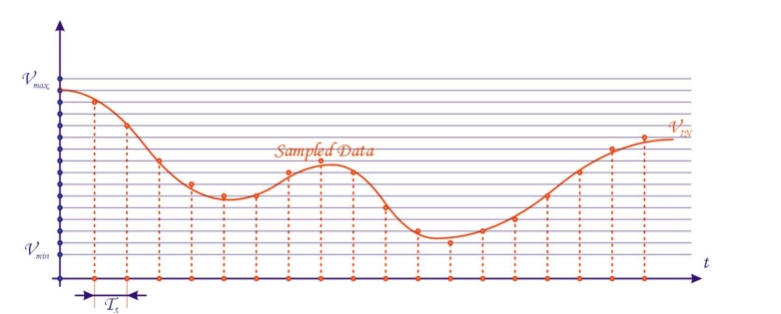
\includegraphics[width=14cm]{figures/ch18/intro1.jpg}
	\caption{}
	\label{fig:intro1}
\end{figure}
An \emph{Analog-to-Digital Converter} (ADC) will convert an analog signal to discrete voltage levels at specific, discrete moments in time. The latter is characterized by the sampling period $T_s$. The reduction to discrete values leads to a quantization error $\epsilon_s$. Preferably, this error should be smaller than the resolution of the measurement. The sampling rate must be higher than the Shannon rate $2 \; \omega_{max}$. If $\omega_{max}$ is unknown or too high (noise!), a low-pass (anti-aliasing) filter must be used.\\
The goal of a data converter is to transfer a signal from the real world to a digital storage device. The signal is picked up by a sensor (an antenna, a microphone, a camera, \ldots ) and will first be sampled by a sample-and-hold circuit, where the present value of the signal is stored on an analog memory (like a capacitor) and then converted by the ADC to a number of bits (a digital \emph{word}) that can be transferred to a digital device for processing and storage. This pipeline is shown in figure \ref{fig:intro2}.\\
\begin{figure}[h!]
	\centering
	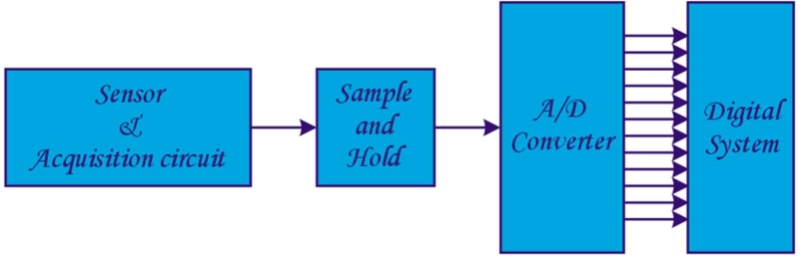
\includegraphics[width=12cm]{figures/ch18/intro2.jpg}
	\caption{}
	\label{fig:intro2}
\end{figure}
This process can also work in the other way: a digital system (like a PC or microcontroller) generates a digital actuator signal. This signal is then converted to an analog signal with a \emph{Digital-to-Analog Converter} (and a filter to smooth out the transitions generated by the conversion process) and is then applied to an actuator.
\begin{figure}[h!]
	\centering
	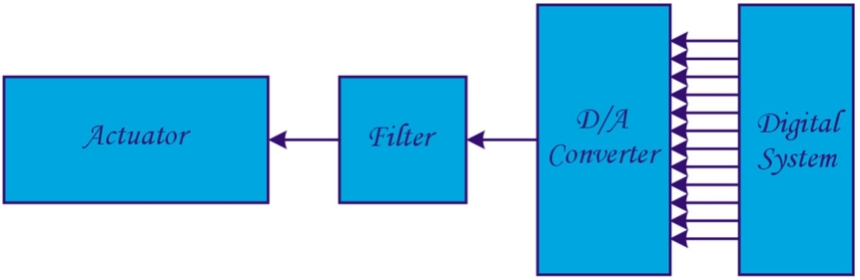
\includegraphics[width=12cm]{figures/ch18/intro3.jpg}
	\caption{}
	\label{fig:intro3}
\end{figure}

\section{Characteristics of DAC \& ADC}
A DAC converts a binary word $b_0 b_1 \ldots b_{n-1}$ of $n$ bits to an analog output $V_{out}$:
$$
V_{out} = \frac{V_{ref}}{2^n} \sum_{i=0}^{n-1} b_i 2^i
$$
as in figure \ref{fig:dac_char1}. The least significant bit (the resolution, or the spacing between two successive analog values) is equal to 
$$
LSB = \frac{V_{ref}}{2^n}
$$
\begin{minipage}{.5\textwidth}
	\centering
	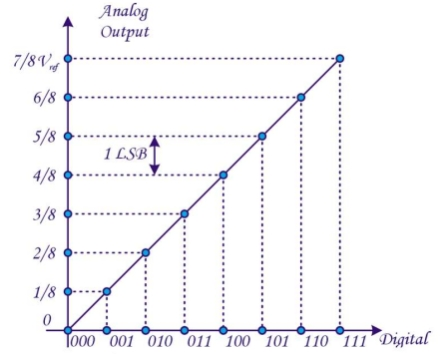
\includegraphics[width=8cm]{figures/ch18/dac_char1.jpg}
	\captionof{figure}{}
	\label{fig:dac_char1}
\end{minipage}%
\begin{minipage}{.5\textwidth}
	\centering
	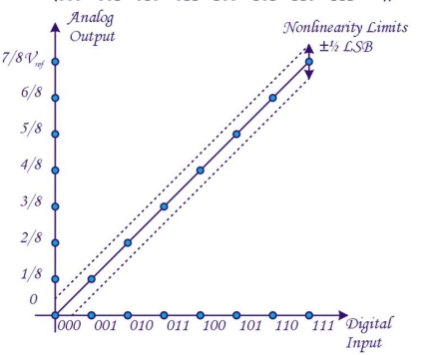
\includegraphics[width=8cm]{figures/ch18/dac_char2.jpg}
	\captionof{figure}{}
	\label{fig:dac_char2}
\end{minipage}
Linearity is important: we require that the error of the generated values is always limited to $\pm$ \nicefrac{1}{2} LSB. If not, it is possible that a code word $a$ that is lower than a code word $b$ produces a higher analog value. \\
A real DAC contains many types or sources of errors beside non-linearity. A true output of a DAC is the red line in figure \ref{fig:dac_char3}, which can be approximated by a best-fit line in blue. This line should keep the error with respect to the real line within \nicefrac{1}{2} LSB. The offset error is the error due to the fact that the best-fit line doesn't go through the origin. Additionally, there is a gain error because the slope is not exactly 1.\\
\begin{figure}[h!]
	\centering
	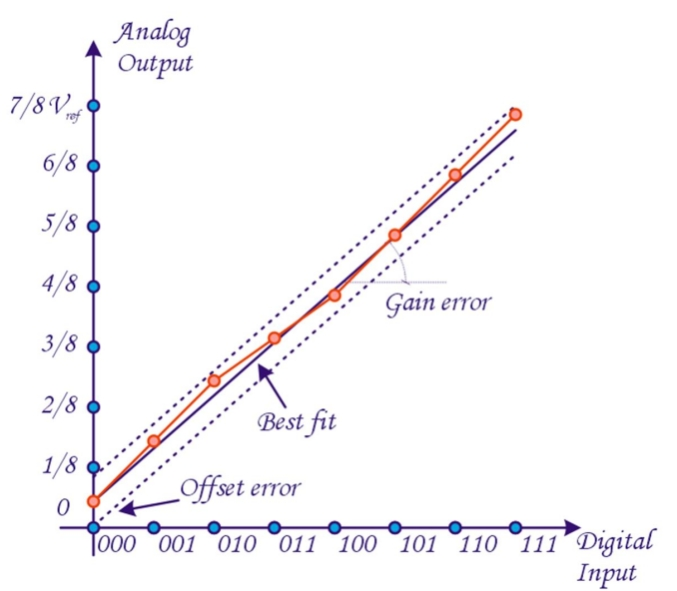
\includegraphics[width=8cm]{figures/ch18/dac_char3.jpg}
	\caption{}
	\label{fig:dac_char3}
\end{figure}
More important are the deviations for each point between the measured line and the best-fit line. The \emph{integral non-linearity} (INL) is the maximum deviation over the whole range, while the \emph{differential non-linearity} (DNL) is the maximum deviation between two consecutive steps: we expect that for one step, the output moves by 1 LSB. The maximal deviation from this LSB is the DNL. The INL gives the linearity, while the DNL determines the resolution. Figures \ref{fig:inl} and \ref{fig:dnl} show DACs with high INL and low DNL (left) and low INL and high DNL (right).\\
\begin{minipage}{.5\textwidth}
	\centering
	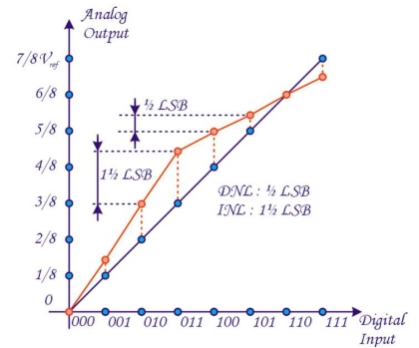
\includegraphics[width=7cm]{figures/ch18/inl.jpg}
	\captionof{figure}{}
	\label{fig:inl}
\end{minipage}%
\begin{minipage}{.5\textwidth}
	\centering
	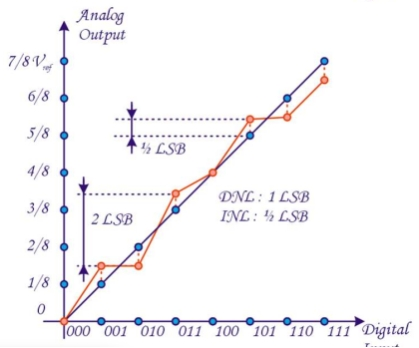
\includegraphics[width=7cm]{figures/ch18/dnl.jpg}
	\captionof{figure}{}
	\label{fig:dnl}
\end{minipage}
An ADC converts analog input value $V_{out}$ into a binary word $b_0 b_1 \ldots b_{n-1}$ of $n$ bits. An example of  an ideal input-output relation with $n=3$ is given in figure \ref{fig:adc_char1}. It follows a staircase pattern where each codeword corresponds to a value of $V_{in}$ between $\frac{k}{2^n} V_{ref} - \frac{1}{2} \frac{1}{2^n} V_{ref}$ and $\frac{k}{2^n} V_{ref} + \frac{1}{2} \frac{1}{2n} V_{ref}$ (except for $000$). The spacing between consecutive codewords is $1$ LSB, as required. The maximum error is $\pm$ \nicefrac{1}{2} LSB.\\
\begin{figure}[h!]
	\centering
	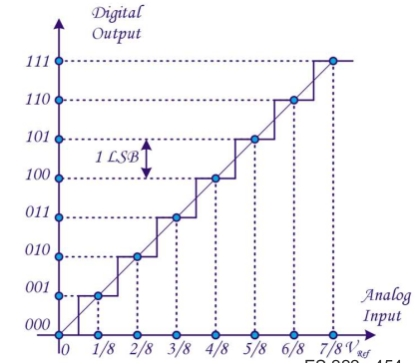
\includegraphics[width=8cm]{figures/ch18/adc_char1.jpg}
	\caption{}
	\label{fig:adc_char1}
\end{figure}
As for the DAC, there is also the notion of INL (global error) and DNL (1-step error). For example, in the left part of figure \ref{fig:adc_char3}, with blue the ideal curve and in red the real one, there is no input value that corresponds with the code "011", so the DNL is high. In the right figure, the relative error of each step is quite small, but there is a significant non-linearity, characterized by a large INL.
\begin{comment}
	
\begin{figure}[h!]
	\centering
	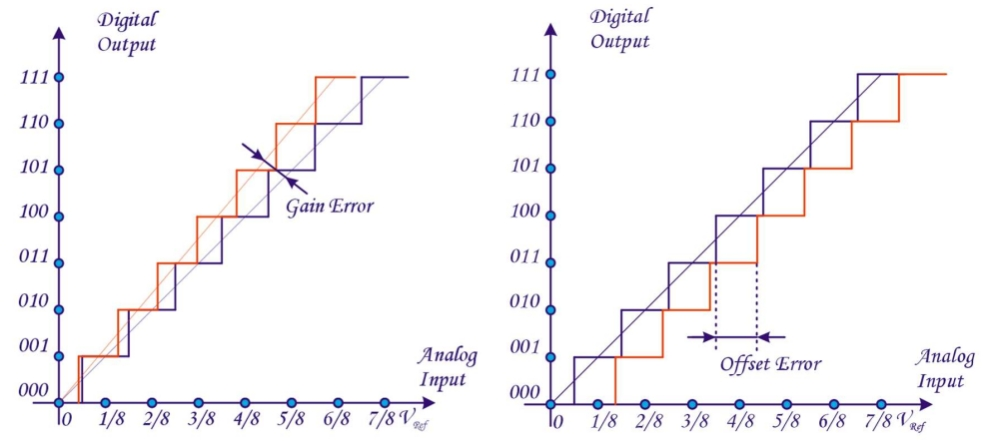
\includegraphics[width=14cm]{figures/ch18/adc_char2.jpg}
	\caption{}
	\label{fig:adc_char2}
\end{figure}
\end{comment}

\begin{figure}[h!]
	\centering
	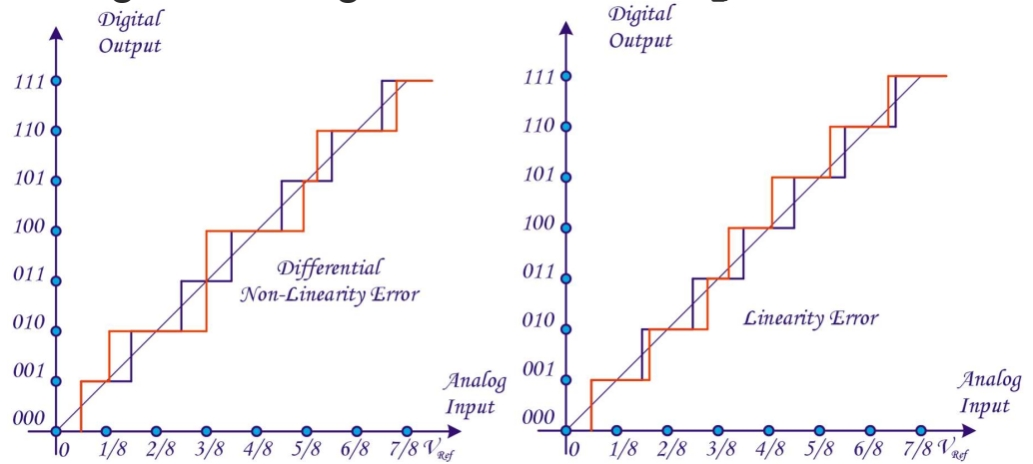
\includegraphics[width=14cm]{figures/ch18/adc_char3.jpg}
	\caption{}
	\label{fig:adc_char3}
\end{figure}

\section{Sample-and-Hold Circuit}
A sample-and-hold circuit temporarily stores the value of an input signal such that it can be processed and converted by an ADC. It consists of a switch, a capacitor and an OPAMP as a unity gain buffer (see chapter \ref{sec:unity_gain_buffer}), as in figure \ref{fig:SH1}.\\
\begin{figure}[h!]
	\centering
	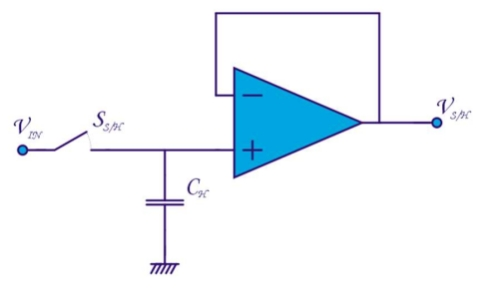
\includegraphics[width=8cm]{figures/ch18/SH1.jpg}
	\caption{}
	\label{fig:SH1}
\end{figure}
During the "Sample"-phase of the cycle (see figure \ref{fig:SH2}, with in red the input signal and in blue the output of the sample-and-hold), the switch is closed. After a transition period $t_A$\footnote{Because the OPAMP and the RC circuit formed by switch and capacitor are a higher order system, there is a settling time and a ripple.} the input of the OPAMP will follow the signal. The time $t_A$ is the \emph{acquisition time}. During the "Hold" part of the cycle, the switch opens and the capacitor will retain the value of the signal at the end of the sample period. During this time, the output $V_{S/H}$ is constant and the ADC can do the conversion. When the input impedance of the OPAMP is not infinite, a small current will be drawn and the voltage on the capacitor will slowly decrease: $\Delta V = \frac{I_{leak}}{C} \Delta t$; this is the \emph{droop rate}.

\begin{figure}[h!]
	\centering
	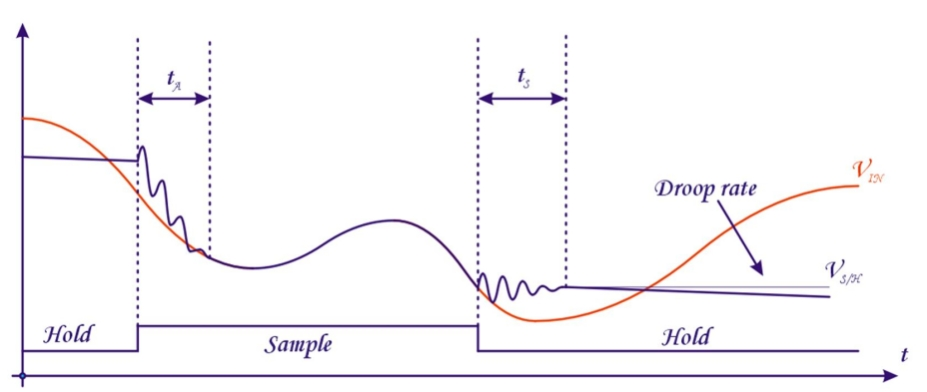
\includegraphics[width=14cm]{figures/ch18/SH2.jpg}
	\caption{}
	\label{fig:SH2}
\end{figure}

\section{Digital-to-Analog Converters}
In this section, we discuss 2 families of DAC's, the first one based on voltage distribution, the other one based on charge distribution. There is a trade-off between precision and speed of conversion.
\subsection{Voltage Distribution}
\label{sec:dac_voltage_distribution}
This converter uses a resistor network to generate the different possible output voltages, as in figure \ref{fig:dac1}. The lowest voltage is $\frac{1}{2} \frac{V_{ref}}{2^n} $, the second level is $\frac{3}{2} \frac{V_{ref}}{2^n} $, and so on. This corresponds to the staircase pattern from figure \ref{fig:adc_char1}. The voltage that is set at the the output is determined by a single switch that is closed while all the other are open. Since each voltage level requires its own switch, the number of switches is $2^n$. To control the switches, the input word $b = b_1 b_2 \ldots b_n$ is converted in a one-hot code as in figure \ref{fig:dac2}.\\
This is a simple solution that works fine and the conversion can happen very fast (a single clock cycle is enough) for a small number of bits. But if we want a $12$-bit decoder, we would need $2^{12} = 4096$ switches and a decoder network that transform a word of $12$ bits into a switch setting containing $4096$ bits, which is far from easy.\\
\begin{minipage}{.6\textwidth}
	\centering
	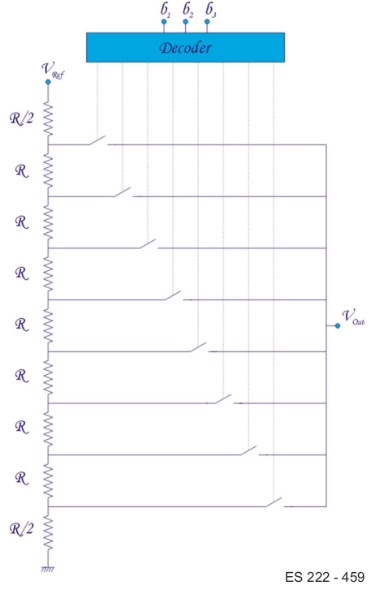
\includegraphics[width=7cm]{figures/ch18/dac1.jpg}
	\captionof{figure}{}
	\label{fig:dac1}
\end{minipage}%
\begin{minipage}{.4\textwidth}
	\centering
	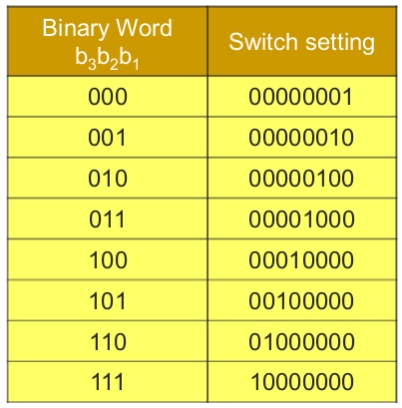
\includegraphics[width=5cm]{figures/ch18/dac2.jpg}
	\captionof{figure}{}
	\label{fig:dac2}
\end{minipage}



\begin{minipage}{.6\textwidth}
	\centering
	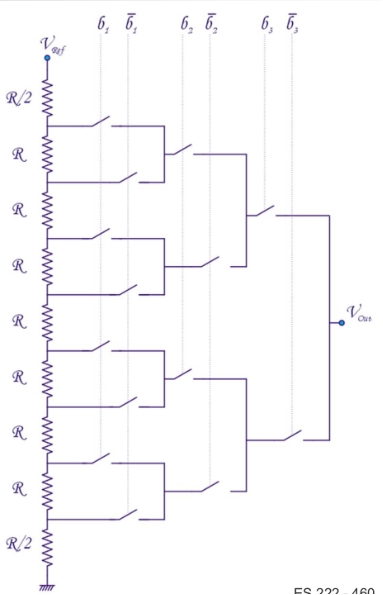
\includegraphics[width=9cm]{figures/ch18/dac3.jpg}
	\captionof{figure}{}
	\label{fig:dac3}
\end{minipage}%
\begin{minipage}{.35\textwidth}
	The complex decoder network for the switch settings can be avoided by implementing a switching network as in figure \ref{fig:dac3}. Note how each bit either opens a one switch or the one below it, because these switches are controlled by $b_i$ or $\overline{b_i}$, respectively.\\
	For every codeword $b$, there will be only one conducting path of closed switches from the resistor network to the output. For instance, if $b = 000$, only in the bottom path are all the switches closed, so $V_{out} = \frac{1}{16} V_{ref}$. If the least significant bit $b_1$ switches from $0$ to $1$, the lowest switch opens but the one just above closes, so now there is a path (and only one path) between $\frac{3}{16} V_{ref}$ and $V_{out}$. If $b_1 = b_2 = b_3 = 1$ there is a path from voltage $\frac{15}{16} V_{ref}$ to $V_{out}$.\\
	 This configuration removes the complexity of the decoder network but requires $\sim 2^{n+1}$ switches.
\end{minipage}

\begin{minipage}{.7\textwidth}
	An elegant solution when a high number of bits is required, is an R-2R-ladder, as in figure \ref{fig:dac4}. Every switch $S_i$ is associated with a bit $b_i$ from the codeword. If the bit is zero, the switch is to ground, and if $b_i = 1$, $S_i$ is at $V_{ref}$.\\
	Assume we want to convert "0001". This means that the three top switches are connected to ground, and the bottom one is at $V_{ref}$. This situation is depicted in figure \ref{fig:dac5} (left). We take the part in the blue square and compute the Thévenin equivalent. Two resistances $2R$ in parallel give $R_{th} = R$, and $E_{th} = \frac{2R}{2R+2R} V_{ref} = \frac{V_{ref}}{2}$, as in the middle part of the figure. With $R$ and $R$ in series, these resistances form one resistance of value $2R$. If we want to transform the blue square in the middle figure, we perform the same calculations and obtain $R_{th} = R$ and $E_{th} = \frac{V_{ref}}{4}$. This process continues, and in the end we find $V_{out} = \frac{V_{ref}}{16}$.\\
	If the codeword is "1000", only the top switch is connected to $V_{ref}$ and all the other ones are at ground. All the resistors at the bottom form parallel combinations of $2R$ with $2R$, which equals $R$. If we keep doing this, we finally find that $V_{out}$ is the output of a voltage divider with two resistances of value $2R$ between $V_{ref}$ and ground, so this means $V_{out} = \frac{2R}{2R + 2R} V_{ref} = \frac{V_{ref}}{2}$.\\
	Try this analysis yourself with the codeword equal to "1010" and see how different voltage levels are added at $V_{out}$.
\end{minipage}
\begin{minipage}{.3\textwidth}
	\centering
	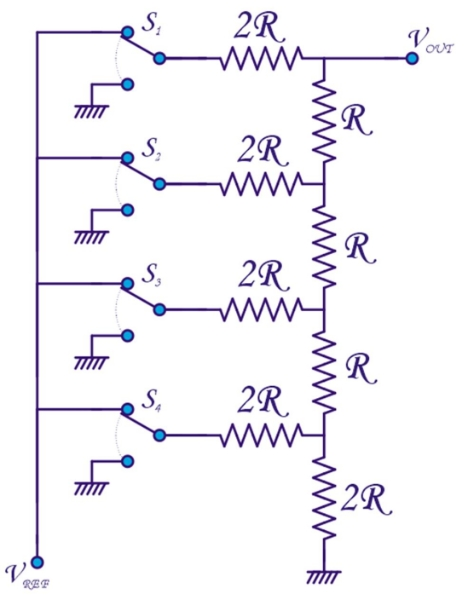
\includegraphics[width=6cm]{figures/ch18/dac4.jpg}
	\captionof{figure}{}
	\label{fig:dac4}
\end{minipage}%

This implementation requires only $n$ switches. The difficulty is creating the resistances with the  right values throughout the whole ladder.
\begin{figure}[h!]
	\centering
	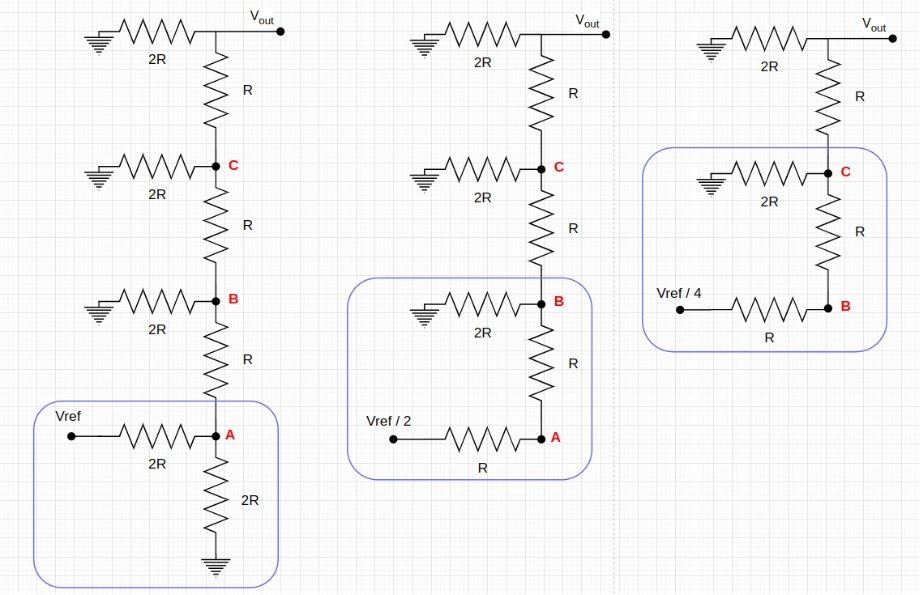
\includegraphics[width=14cm]{figures/ch18/dac5.jpg}
	\caption{}
	\label{fig:dac5}
\end{figure}

\subsection{Charge Distribution}
\label{sec:charge_distribution}
The DAC's from the previous section all worked by creating the different voltage levels are transforming them via a network of switches ot the output. The DAC's we'll study now accumulate charges over a network of capacitors to create the required voltage at the output. To implement this, we use the circuit from figure \ref{fig:dac6}, with $5$ capacitors in parallel. Because there are $4$ switches $S_1$ to $S_4$, this is a $4$-bit DAC.\\

\begin{figure}[h!]
	\centering
	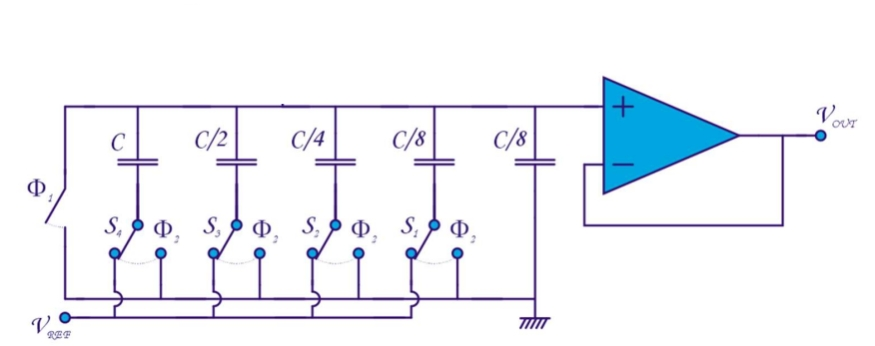
\includegraphics[width=12cm]{figures/ch18/dac6.jpg}
	\caption{}
	\label{fig:dac6}
\end{figure}

During the first phase of the cycle, all switches are closed i.e. connected to ground, so the different capacitors are all discharged. During the second phase of the cycle, switch $S_i$ is connected to $V_{ref}$ if $b_i = 1$ and to ground if $b_i = 0$. The equivalent capacitance $C_{eq}$ from $V_{ref}$ to the positive input of the OPAMP is:
$$
C_{eq} = \sum_{i=1}^{n} b_i \frac{C}{2^{n-i}} = \frac{C}{2^n} \sum_{i=1}^{n} b_i 2^i
$$

\begin{minipage}{.5\textwidth}
	Figure \ref{fig:dac7} on the right shows the simplified circuit, with $V_{out}$ as the result of voltage divider with $C_{eq}$ and $2C-C_{eq}$ (because $C_{tot} = 2 C$). So:
	\begin{align*}
		I = j\omega C_{eq} (V_{ref} - V_{out}) &= j \omega (C_{tot}-C_{eq}) V_{out} \\
		\Rightarrow V_{out} = \frac{C_{eq}}{C_{tot}} &= \frac{V_{ref}}{2^{n+1}} \sum_{i=1}^n b_i 2^i 
	\end{align*}
\end{minipage}
\begin{minipage}{.5\textwidth}
	\centering
	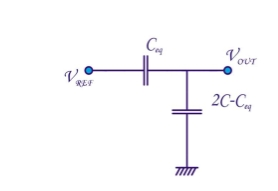
\includegraphics[width=7cm]{figures/ch18/dac7.jpg}
	\captionof{figure}{}
	\label{fig:dac7}
\end{minipage}\\
This means that every bit equal to $1$ contributes a fraction of $V_{ref}$ to the output voltage $V_{out}$ in proportion to its value $2^i$, just as required. \\
In practice, it can be difficult to make such small capacitances with high enough precision - knowing that the maximum error we may make is one LSB. A potential solution to this problem is the use of a shunt capacitance $C_{shunt}$ as in the $6$-bit converter of figure \ref{fig:dac8}. At the right of $C_{shunt}$, the total capacitance we see is $C + C/2 + C/4 + C/4 = 2C$, but we actually want to see $C/4$ from the left of $C_{shunt}$, looking to the right. With $C_{shunt}$ in series with the total right capacitance $2C$ and the expression for two capacitances in series, we can compute $C_{shunt}$:
$$\frac{C}{4} = \frac{C_{shunt} \; 2C}{C_{shunt} + 2C}$$
with result $C_{shunt} = \frac{8}{7} \frac{C}{4} = \frac{2}{7} C$ as indicated in the figure. This solution, maybe repeated several times, allows to make precise converters with a resolution of several bits. Note however that each conversion is a two-step process: first the capacitors are discharges, and after that only the capacitors with bits equal to $1$ are connected to $V_{ref}$.

\begin{figure}[h!]
	\centering
	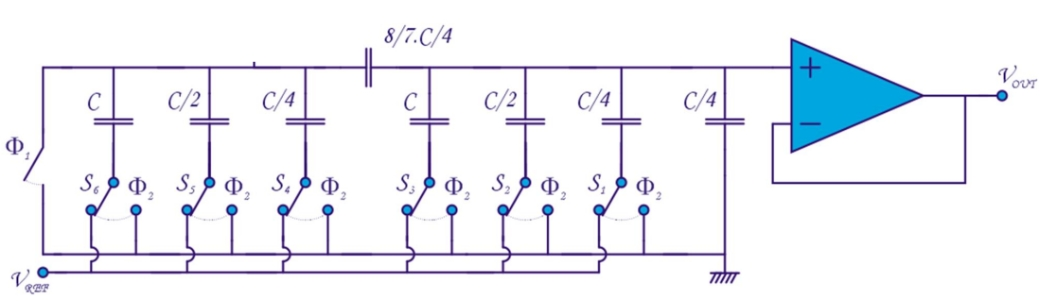
\includegraphics[width=16cm]{figures/ch18/dac8.jpg}
	\caption{}
	\label{fig:dac8}
\end{figure}

\subsection{Serial Charge Distribution}
\label{sec:serial_charge}
Instead of having a capacitor for each bit, we can also charge a single capacitor every time a bit is high. The circuit used for this digital-to-analog conversion is shown in figure \ref{fig:dac9}.\\

\begin{figure}[h!]
	\centering
	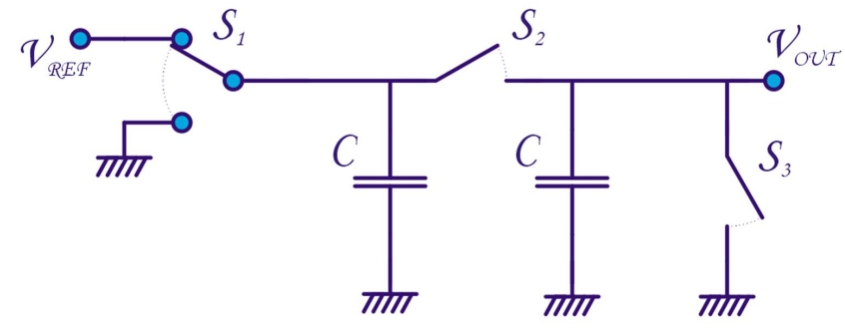
\includegraphics[width=12cm]{figures/ch18/dac9.jpg}
	\caption{}
	\label{fig:dac9}
\end{figure}

Initially, all switches are closed (with $S_1$ connected to ground) so that all capacitors can discharge. Then the conversion happens in $n$ cycles for each of the $b_i$ bits:
\begin{enumerate}
	\item With switch $S_2$ open, switch $S_1$ is set to ground if $b_i = 0$ or to $V_{ref}$ if $b_i = 1$. The charge on the first capacitor $C$ is then $b_i \; C \; V_{ref}$, irrespective of the charge that was on it before.
	\item Switch $S_1$ is reopened - this means it connects to neither ground or $V_{ref}$.
	\item Switch $S_2$ is closed and reopened. This means that the charge that was present of the first and second capacitor is now equally distributed over both. So the charge on the second capacitor is now:
	$$ Q_{new} = \frac{Q_{old} + b_i C V_{ref}}{2} $$
	\item This procedure continues until the last bit is evaluated.
\end{enumerate}
So after $n$ cycles, the total charge on the second capacitor is $Q = \sum_{i=1}^n \frac{b_i C V_{ref}}{2^i}$ and so
 $$V_{out} = Q/C =  \frac{V_{ref}}{2^{n+1}} \sum_{i=1}^{n} b_i 2^i$$
 which is exactly what we need. This DAC can be easily constructed and can be very precise, but it will be slow because it requires $n+1$ cycles (including the discharge) to convert a word of length $n$.

\section{Analog-to-Digital Converters}
\subsection{Serial Converter}
\label{sec:serial_adc}
The circuit of a  serial converter is shown in figure \ref{fig:adc1}. The first OPAMP, with a constant input voltage $V_{ref}$, is an integrator: $i = -V_{REF} / R  = (-V_o) j \omega C$ so $$V_O(j\omega)  = \frac{1}{j \omega RC} V_{REF} \Leftrightarrow v_o(t)= \int_{0}^{\Delta t} \frac{1}{RC} V_{REF} \; dt = \frac{1}{RC} V_{REF} \; \Delta t$$
This linearly rising signal is compared by the second OPAMP with the input signal (from the sample-and-hold) $V_{IN}$. As long as $V_{IN}$ is higher than the ramp, the output is high, and once the ramp passes $V_{IN}$, the output goes low. The result is a block signal whose length is proportional to $V_{IN}$. \\
This signal is applied at an AND-gate with a clock signal of frequency $f = \frac{1}{T}$ at the other input. The output of the AND-gate will be the clock as long as the signal is high, and low when the signal is low.  The result is a sequence of pulses whose number $N$ is proportional to $V_{IN}$. These pulses are counted by counter to produce the binary out signal.\\
The length of the signal at the output of the comparator is thus $N T$, reached when $V_{IN}$ is equal to the ramp signal, and subsequently
$$
V_{IN} = N T \frac{V_{REF}}{RC}
$$
with the LSB equal to $T \frac{V_{REF}}{RC}$. This is a very precise conversion; the most likely sources of error are a change in $R$ and $C$ because the circuit heats up, or drift of the clock. The disadvantage is that conversion takes $2^n$ clock cycles, which can be prohibitively large.
\begin{figure}[h!]
	\centering
	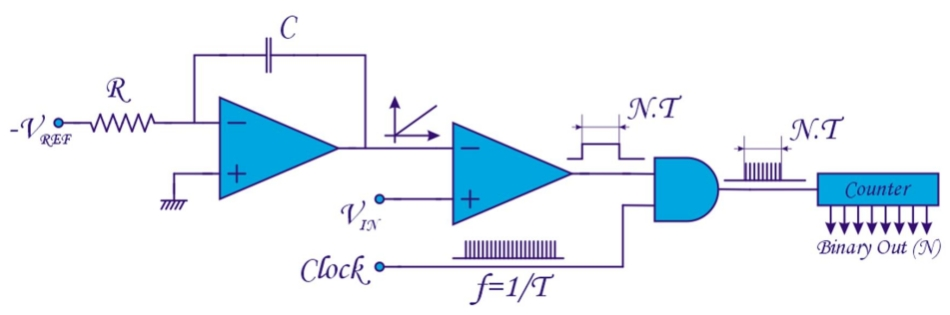
\includegraphics[width=14cm]{figures/ch18/adc1.jpg}
	\caption{}
	\label{fig:adc1}
\end{figure}

\subsection{Double Integration}
A solution to work even more precisely, is the double integration scheme from figure \ref{fig:adc2}. At the input, there is switch that either places $V_{IN}$ or $-V_{REF}$ at the input of the integrator. Initially, it will be $V_{IN}$ and at the output of the integrator, we have a linearly decreasing signal whose slope is determined by the value of $V_{IN}$: $- \frac{V_{IN}}{RC}$. After $N_{REF}$ clock cycles, the digital controller will put the switch at $-V_{REF}$.The signal at the output of the integrator is then $-\frac{V_{IN}}{RC} N_{REF} T + V_{th}$.\\
From that point on, the integration will be in the other direction, with a fixed sloped determined by $V_{REF}$, as in figure \ref{fig:adc3}. After a time $NT$, the threshold voltage $V_{th}$ is reached and the output of the comparator goes low. At that time, we have:
$$
\frac{V_{IN}}{RC} N_{REF} T = \frac{V_{REF}}{RC} N T \Leftrightarrow N = \frac{1}{N_{REF}}\frac{V_{IN}}{V_{REF}}
$$
\begin{figure}[h!]
	\centering
	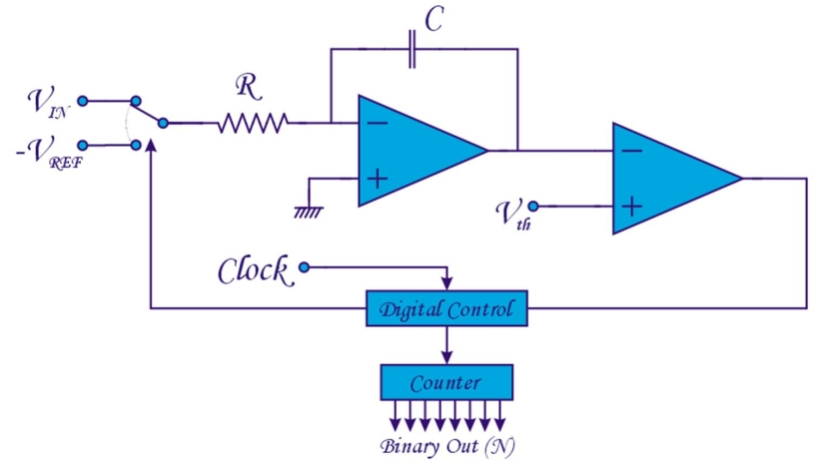
\includegraphics[width=14cm]{figures/ch18/adc2.jpg}
	\caption{}
	\label{fig:adc2}
\end{figure}
In this way, the dependence on $R$, $C$ and the clock period is removed. The LSB is $\frac{V_{REF}}{N_{REF}}$. The disadvantage is the same as before: conversion takes $2^n$ clock cycles and for some applications this can be too long.
\begin{figure}[h!]
	\centering
	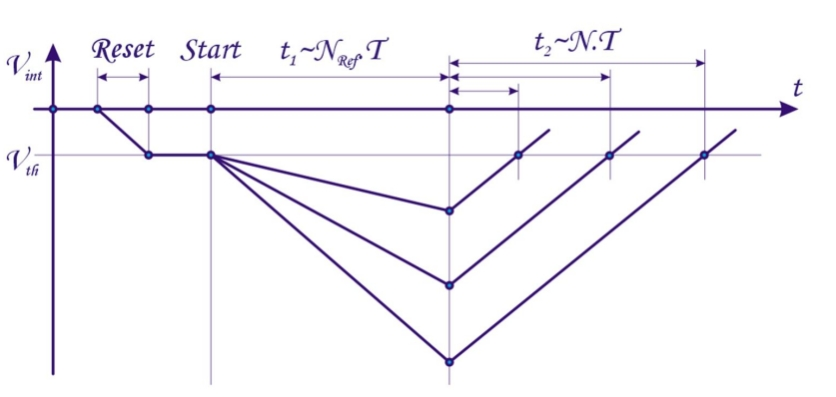
\includegraphics[width=14cm]{figures/ch18/adc3.jpg}
	\caption{}
	\label{fig:adc3}
\end{figure}

\subsection{Successive Approximation}
\label{sec:sar}
A SAR or \emph{Successive Approximation Register} performs a binary search over the space of codewords such that the corresponding voltage approximates the input voltage $V_{IN}$. The circuit is given in figure \ref{fig:adc4a}.\\

\begin{minipage}{.6\textwidth}
	\centering
	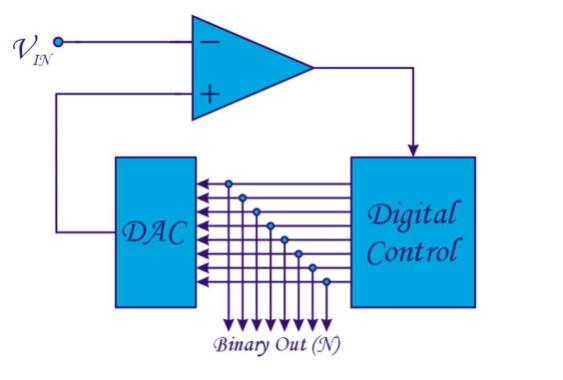
\includegraphics[width=9cm]{figures/ch18/adc4a.jpg}
	\captionof{figure}{}
	\label{fig:adc4a}
\end{minipage}%
\begin{minipage}{.4\textwidth}
	\centering
	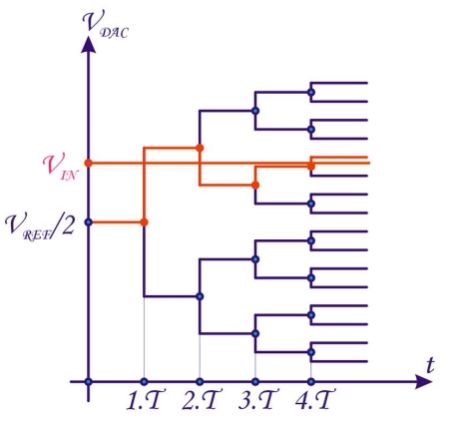
\includegraphics[width=6cm]{figures/ch18/adc4b.jpg}
	\captionof{figure}{}
	\label{fig:adc4b}
\end{minipage}

The digital controller generates a code that is transformed by the DAC into a voltage that is compared with the input $V_{IN}$ by the comparator. Suppose the initial code was "1000". This generates a voltage in the middle of the domain, $\frac{1}{2} V_{REF}$. If the input signal is higher - as in figure \ref{fig:adc4b}, the output of the comparator is low and the controller knows the first "1" is correct. If the input were lower, the first bit (the most significant bit) must be a "0". During the next clock cycle, the digital controller will generate a code word "1100", the DAC will generate the corresponding voltage. This voltage is too high, as the figure shows, so the second bit will be a "0". This continues for the remaining bits. The correct codeword for this example is "10110".\\
This is a simple and straightforward converter that only needs $n$ clock cycles to convert a signal to an $n$-bit word, but it requires a digital-to-analog converter and is (because of this DAC) less accurate.

\subsection{Flash Converter}
\label{sec:flash}
\begin{minipage}{.5\textwidth}
	Figure \ref{fig:adc5} on the right shows the \emph{flash converter}, so-called because it's a very fast analog-to-digital converter.\\
	It works by generating all $2^n$ voltage levels between $0$ and $V_{REF}$ with a voltage ladder, just as the voltage distribution DAC from section \ref{sec:dac_voltage_distribution}. With $2^n$ comparators, the input voltage $V_{IN}$ is compared with each voltage level. The output of all comparators at a voltage lower than $V_{IN}$ will be one and the output of all those who lie higher will be zero. This is the so-called \emph{thermometer code} that is transformed by the digital decoder network in a codeword of $n$ bits.\\
	This converter is very fast: it does the conversion in a single clock cycle, but it is not very accurate and requires a lots of components: $2^n$ resistors, $2^n$ comparators, each with an offset voltage that must be kept lower than 1 LSB, and a decoder network with $2^n$ inputs and $n$ outputs. Construction of this converter is only feasible for $n \le 10$.
\end{minipage}
\begin{minipage}{.5\textwidth}
	\centering
	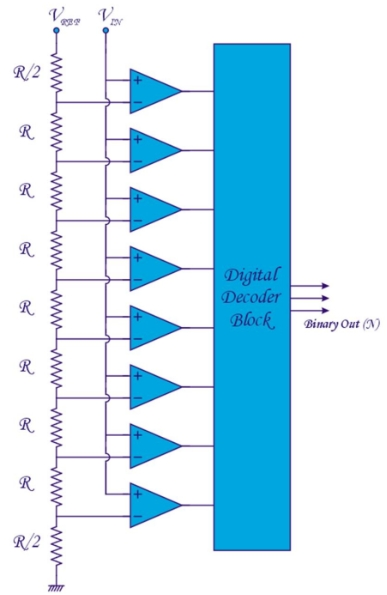
\includegraphics[width=7cm]{figures/ch18/adc5.jpg}
	\captionof{figure}{}
	\label{fig:adc5}
\end{minipage}\\

\subsection{2-Step Flash}
In stead of making a single $N$-bit flash converter, we can also make two consecutive $N/2$-bit converters, as in figure \ref{fig:adc6}. The first ADC of size $N/2$ creates the first $N/2$ most significant bits of the output code word. These bits are then converted by a $N/2$ DAC to a voltage that is subtracted from the input signal. The range of this residual voltage is a single LSB of the first converter. A second ADC of size $N/2$, tuned to this range of 1 LSB, converts the residual signal to an $N/2$ codeword. This word constitutes the $N/2$ least significant bits of the $N$-bit codeword. In this way, the complexity is reduced: from $2^N$ to $2 \times 2^{N/2}$.
\begin{figure}[h!]
	\centering
	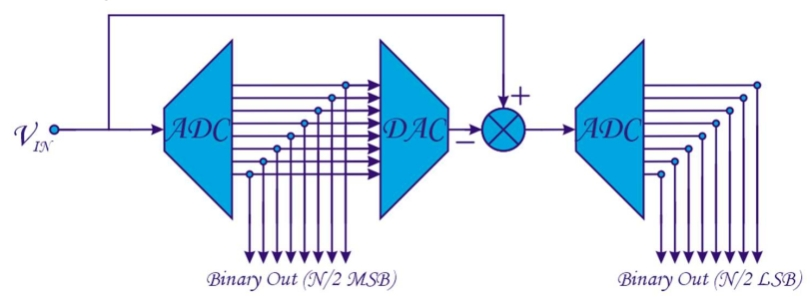
\includegraphics[width=14cm]{figures/ch18/adc6.jpg}
	\caption{}
	\label{fig:adc6}
\end{figure}

\subsection{Pipeline Converter}

A \emph{pipeline converter} takes the idea from the 2-step flash converter even further: we convert a single bit at a time. Figure \ref{fig:adc7} shows a $3$-bit pipeline. In the first comparator, we compare $V_{IN}$ with $V_{REF}$ - note that in this case, the range is $2\;V_{REF}$, so $V_{REF}$ is exactly in the middle. MSB $b_1$ will be $1$ if $V_{IN}$ is higher and zero otherwise. To compute the residual - as in figure \ref{fig:adc6} - we don't use a DAC because with a single bit, we subtract either $V_{REF}$ or ground from $V_{IN}$ - hence the switch after the comparator, which is controlled by $b_1$. The next step would be to compare the residual with $\frac{1}{2} V_{REF}$. But this would require the generation of $\frac{V_{REF}}{2}$ and later $\frac{V_{REF}}{4}$, $\frac{V_{REF}}{8}$, etc \ldots. To avoid this, we multiply the residual by two and compare with $V_{REF}$ - an operation that gives the same result and avoids all these intermediary reference levels. This comparison gives $b_2$ and the same process continues.\\
This is a pipeline because the different stages can work independently from each other: after the first bit of sample $1$ is converted, the conversion goes on but the first stage is now ready to convert the first bit of sample $2$. So after $n$ clock cycles, the first sample is completely converted, but after that there will be a new codeword after each clock period, because the samples move through the pipeline.

\begin{figure}[h!]
	\centering
	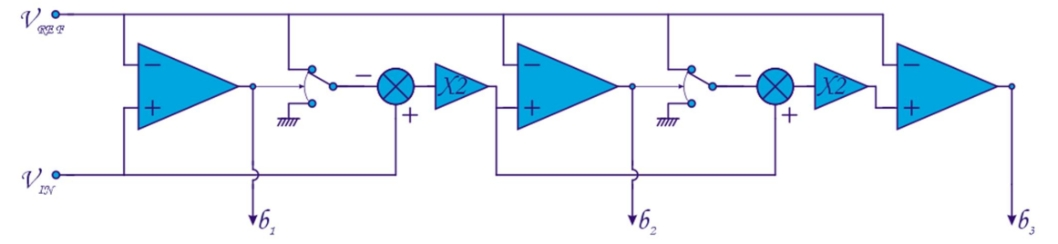
\includegraphics[width=15cm]{figures/ch18/adc7.jpg}
	\caption{}
	\label{fig:adc7}
\end{figure}

\section{Additional Notes}
In general, for both DACs and ADCs, we can state that the accuracy is inversely proportional to the speed: the more accuracy you require, the slower the conversion will be. For ADCs, we find:
\begin{itemize}
	\item Serial converter: low speed, precision of $12-14$ bits.
	\item SAR converter: medium speed, $10 - 12$ bits.
	\item Flash converter: highest speed, $8-10$ bits
\end{itemize}
Anything over 14 bits bits will require special techniques, outside the scope of this course.\\
A figure-of-merit for ADC is defined to compare converters with a single number:
$$FOM = \frac{P}{2^n f_c}$$
with $P$ the power dissipation, $f_c$ the conversion speed and $n$ the number of bits. At this time, the best FOM $\sim 50 nJ$.
